\documentclass[10pt]{standalone}
\usepackage{times}
\usepackage{amsmath,amssymb,xspace,xcolor,tikz}
\usetikzlibrary{arrows.meta,positioning,shapes.geometric,calc,fit,backgrounds,decorations.pathmorphing}

\newcommand{\todo}[1]{{\color{red}#1}}
\newcommand{\TODO}[1]{\textbf{\color{red}[TODO: #1]}}
\newcommand{\method}{CxWM\xspace}
\newcommand{\vjepa}{V-JEPA~2.1\xspace}
\newcommand{\flywire}{FlyWire\xspace}
\providecommand{\etal}{\emph{et al}.\xspace}
\providecommand{\ie}{\emph{i.e}.\xspace}
\providecommand{\eg}{\emph{e.g}.\xspace}
\newcommand{\degree}{$^\circ$}
\let\mathpm\pm
\renewcommand{\pm}{\ensuremath{\mathpm}}

% diagram colours (populations match the released 3-D viewer)
\definecolor{cVIS}{RGB}{66,133,244}
\definecolor{cCX}{RGB}{244,160,0}
\definecolor{cMB}{RGB}{52,168,83}
\definecolor{cOUT}{RGB}{219,68,155}
\definecolor{cTeach}{RGB}{90,90,90}
\tikzset{
  box/.style={draw,rounded corners=2pt,minimum height=1.6em,inner sep=4pt,font=\small,align=center},
  pop/.style={box,fill=#1!15,draw=#1!80!black,thick},
  arr/.style={-{Latex[length=2mm]},thick},
  darr/.style={-{Latex[length=2mm]},thick,dashed},
  lbl/.style={font=\scriptsize,align=center},
}
\begin{document}
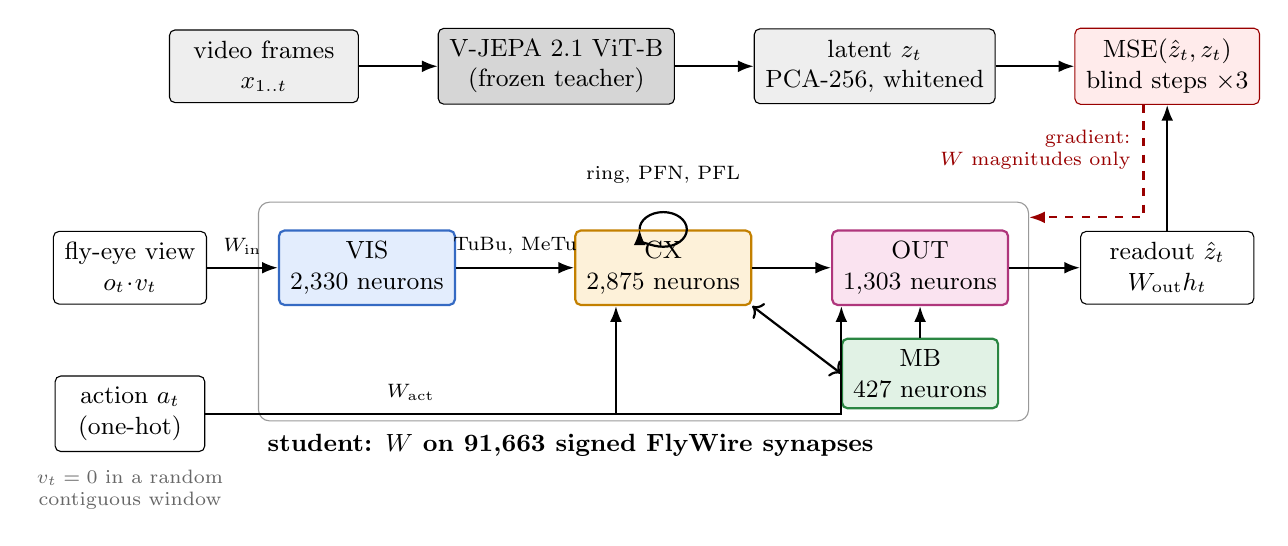
\begin{tikzpicture}[node distance=6mm and 10mm]
    % student row
    \node[pop=cVIS,minimum width=2.2cm] (vis) {VIS\\2,330 neurons};
    \node[pop=cCX,right=15mm of vis,minimum width=2.2cm] (cx) {CX\\2,875 neurons};
    \node[pop=cOUT,right=of cx,minimum width=2.2cm] (out) {OUT\\1,303 neurons};
    \node[pop=cMB,below=4mm of out,minimum width=1.6cm] (mb) {MB\\427 neurons};
    \draw[arr] (vis) -- node[lbl,above=1pt]{TuBu, MeTu} (cx);
    \draw[arr] (cx) -- (out);
    \draw[arr,<->] (cx.south east) -- (mb.west);
    \draw[arr] (mb.north) -- (out.south);
    \draw[arr] (cx.north) ++(-3mm,0) arc (180:-180:3mm and 2.2mm);
    \node[lbl,anchor=south] at ([yshift=4.6mm]cx.north) {ring, PFN, PFL};
    \begin{scope}[on background layer]
      \node[draw=black!40,rounded corners,fit=(vis)(cx)(mb)(out),inner sep=7pt,yshift=1mm] (student) {};
    \end{scope}
    \node[font=\small\bfseries,anchor=north west] at ([yshift=-1pt]student.south west) {student: $W$ on 91,663 signed \flywire synapses};
    % inputs
    \node[box,left=9mm of vis,minimum width=1.9cm] (eye) {fly-eye view\\$o_t\!\cdot\!v_t$};
    \draw[arr] (eye) -- node[lbl,above=1pt]{$W_{\rm in}$} (vis);
    \node[box,below=9mm of eye,minimum width=1.9cm] (act) {action $a_t$\\(one-hot)};
    \draw[arr] (act.east) -| node[lbl,pos=.25,above=1pt]{$W_{\rm act}$} ([xshift=-6mm]cx.south);
    \draw[arr] (act.east) -| ([xshift=-10mm]out.south);
    \node[lbl,below=1mm of act,text=black!60] {$v_t=0$ in a random\\contiguous window};
    % readout, loss, teacher row
    \node[box,right=9mm of out,minimum width=2.2cm] (hat) {readout $\hat z_t$\\$W_{\rm out} h_t$};
    \draw[arr] (out) -- (hat);
    \node[box,fill=red!8,draw=red!60!black,above=16mm of hat,minimum width=2.2cm] (loss) {MSE$(\hat z_t, z_t)$\\blind steps $\times 3$};
    \draw[arr] (hat) -- (loss);
    \node[box,fill=cTeach!10,left=of loss,minimum width=2.4cm] (z) {latent $z_t$\\PCA-256, whitened};
    \node[box,fill=cTeach!25,left=of z,minimum width=2.6cm] (vjepa) {\vjepa ViT-B\\(frozen teacher)};
    \node[box,fill=cTeach!10,left=of vjepa,minimum width=2.4cm] (frames) {video frames\\$x_{1..t}$};
    \draw[arr] (frames) -- (vjepa);
    \draw[arr] (vjepa) -- (z);
    \draw[arr] (z) -- (loss);
    \draw[darr,red!60!black] (loss.south) ++(-3mm,0) |- node[lbl,pos=.2,left=1pt,align=right]{gradient:\\$W$ magnitudes only} ([yshift=-2mm]student.north east);
  \end{tikzpicture}
\end{document}
